\subsubsection{CNN Results}
\label{sec:cnn_results}

The CNN machine learning model was trained, as mentioned in the methodology, which allowed us to obtain a total of 3,203,969 parameters for training. After 16 epochs, the values shown in Table~\ref{tab:train_metrics} were obtained for the training and validation phases. Training stopped at epoch 16 due to early stopping. However, the final results evaluated on the test data are presented in Table~\ref{tab:test_metrics}.

We can observe that, compared to previous studies on which our work is based, the accuracy was lower; nonetheless, the obtained results indicate that overfitting was avoided during training and a proper balance between training and validation phases was achieved.

\begin{table}[h]
    \centering
    \caption{Metrics during training and validation (final epoch)}
    \label{tab:train_metrics}
    \begin{tabular}{lcc}
        \toprule
        Metric         & Training & Validation \\
        \midrule
        Accuracy       & 0.8850   & 0.8624     \\
        Loss           & 0.2608   & 0.3153     \\
        Precision      & 0.9340   & 0.9150     \\
        Recall         & 0.8344   & 0.8065     \\
        \bottomrule
    \end{tabular}
\end{table}

\begin{table}[h]
    \centering
    \caption{Final metrics on test data}
    \label{tab:test_metrics}
    \begin{tabular}{lc}
        \toprule
        Metric    & Value   \\
        \midrule
        Accuracy  & 0.8618  \\
        Precision & 0.9266  \\
        Recall    & 0.7929  \\
        F1 Score  & 0.8546  \\
        \bottomrule
    \end{tabular}
\end{table}

ssss

As shown in Figure~\ref{fig:cnn_accuracy}, the training accuracy was initially lower than the validation accuracy during the early epochs. However, the difference was not substantial—approximately four percentage points. Around epoch 16, this trend reversed, with training accuracy surpassing validation accuracy. Despite this shift, an early stopping mechanism was applied to prevent overfitting by halting the training process once the validation performance ceased to improve significantly.

\begin{figure}[H]
    \centering
    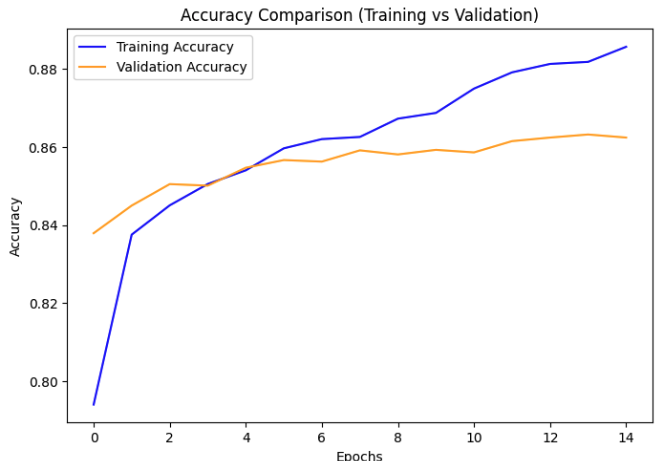
\includegraphics[width=0.45\textwidth]{images/AccuracyComparisonCNN.png}
    \caption{Accuracy comparison between training and validation for CNN model}
    \label{fig:cnn_accuracy}
\end{figure}

A similar but inverse trend can be observed in the loss curves, as shown in Figure~\ref{fig:cnn_loss}. At the beginning of training, the training loss is higher than the validation loss, with a nominal difference of approximately 0.1. As training progresses, this behavior reverses, and the training loss becomes lower than the validation loss. This indicates that while the model initially struggles more with the training data, it gradually learns to generalize, although the growing gap at later epochs may hint at overfitting, which was mitigated by applying early stopping.

\begin{figure}[H]
    \centering
    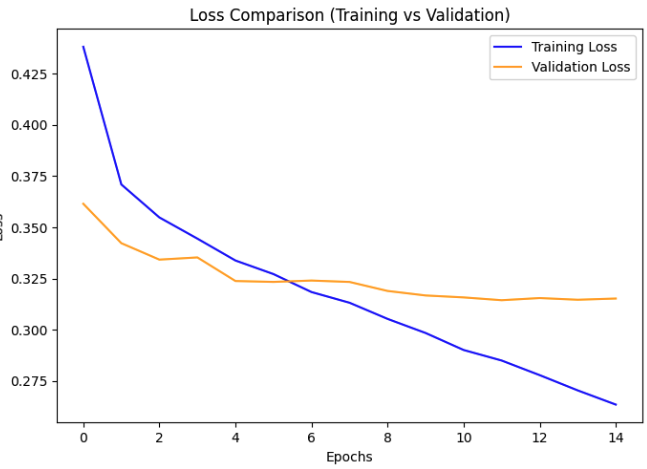
\includegraphics[width=0.45\textwidth]{images/LossComparisonCNN.png}
    \caption{Loss comparison between training and validation for CNN model}
    \label{fig:cnn_loss}
\end{figure}

In the case of precision, as shown in Figure~\ref{fig:cnn_precision}, we observe a gradual increase beginning around the second epoch. However, the precision values for the validation set fluctuate between 89\% and 94\%. This variability may be primarily attributed to the limited amount of training data available. Nevertheless, the achieved precision values can be considered favorable and promising for potential deployment in a production setting.

\begin{figure}[H]
    \centering
    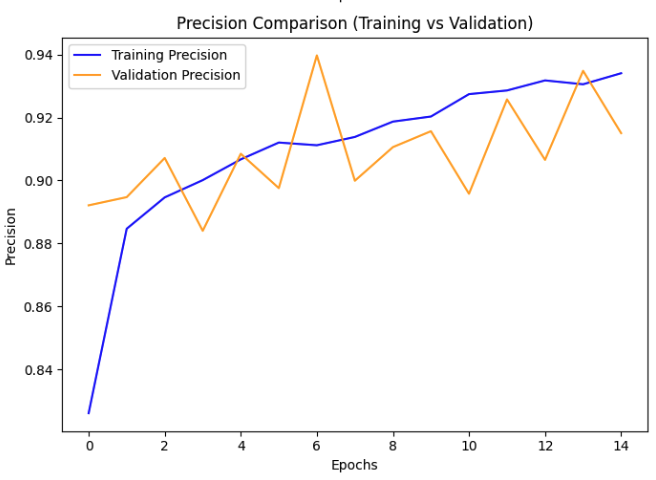
\includegraphics[width=0.45\textwidth]{images/PrecisionComparisonCNN.png}
    \caption{Precision comparison between training and validation for CNN model}
    \label{fig:cnn_precision}
\end{figure}

The recall metric, illustrated in Figure~\ref{fig:cnn_recall}, exhibits a consistent and positive upward trend during training. However, the validation recall demonstrates a more oscillatory behavior, fluctuating throughout the epochs. This variation in the validation set may indicate sensitivity to the limited dataset or variability in the model's ability to generalize recall performance.

\begin{figure}[H]
    \centering
    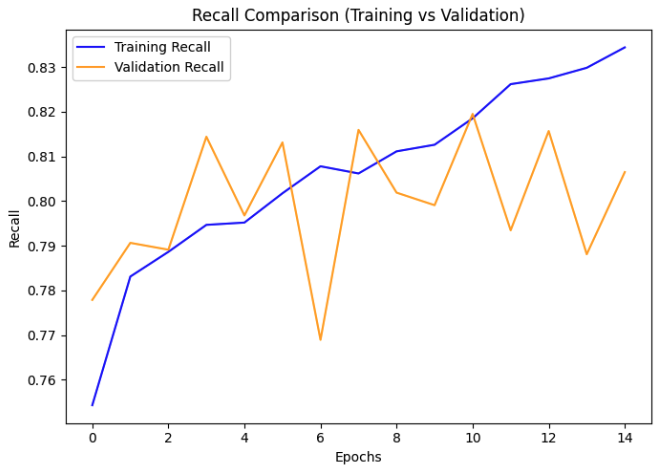
\includegraphics[width=0.45\textwidth]{images/RecallComparisonCNN.png}
    \caption{Recall comparison between training and validation for CNN model}
    \label{fig:cnn_recall}
\end{figure}
 
The confusion matrix shows that the model correctly classifies 4,347 cases as "No hate speech" and 3,875 cases as "Hate speech." However, it also presents 307 false positives (cases wrongly labeled as hate speech when they are not) and 1,012 false negatives (hate speech cases not detected). This imbalance indicates that, although the model is quite accurate, there is still significant room for improvement in detecting hate speech and reducing false negatives, which can have a considerable impact on automatic moderation.

\begin{figure}[H]
    \centering
    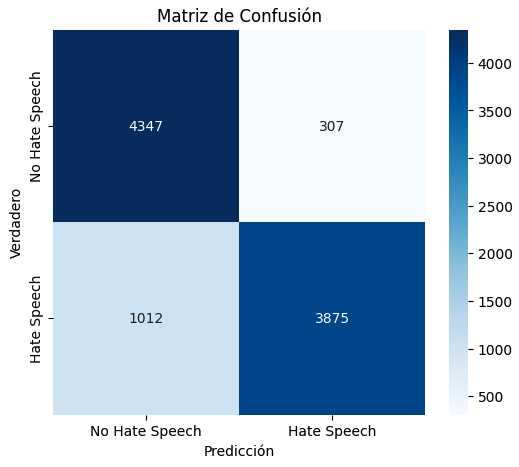
\includegraphics[width=0.45\textwidth]{images/matrixOfConfusion.png}
    \caption{Confusion matrix of the model's predictions on the test set.}
    \label{fig:confusion_matrix}
\end{figure}
